\documentclass{standalone}
\usepackage{tikz}
\begin{document}
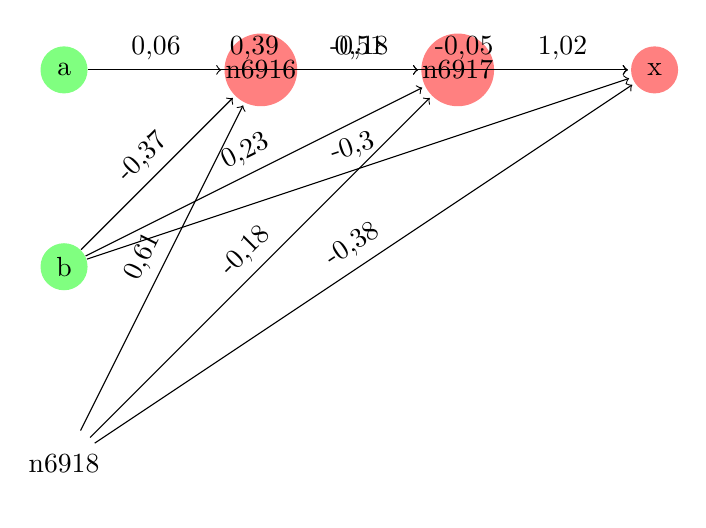
\begin{tikzpicture}[shorten >=1pt,->,draw=black!,node distance=2.5cm]
\tikzstyle{neuron}=[circle,fill=black!25,minimum size=17pt,inner sep=0pt]
\tikzstyle{constant}=[neuron, fill=white!50];
\tikzstyle{identity}=[neuron, fill=green!50];
\tikzstyle{sigmoid}=[neuron, fill=red!50];
\node [identity] (a) {a};
\node [identity,below of=a] (b) {b};
\node [constant,below of=b] (n6918) {n6918};
\node [sigmoid,right of=a] (n6916) {n6916};
\node [sigmoid,right of=n6916] (n6917) {n6917};
\node [sigmoid,right of=n6917] (x) {x};
\path[every node/.style={sloped,anchor=south,auto=false}]
(b) edge node {-0,37} (n6916)
(b) edge node {0,23} (n6917)
(b) edge node {-0,3} (x)
(a) edge node {-0,18} (x)
(a) edge node {0,06} (n6916)
(a) edge node {0,39} (n6917)
(n6917) edge node {1,02} (x)
(n6918) edge node {-0,38} (x)
(n6918) edge node {-0,18} (n6917)
(n6918) edge node {0,61} (n6916)
(n6916) edge node {0,51} (n6917)
(n6916) edge node {-0,05} (x)
;\end{tikzpicture}
\end{document}